\section{Conceitos iniciais: tensão, corrente e potência}

\begin{frame}{Introdução}
	\begin{block}{}
		\begin{itemize}
			\item Você já se perguntou como são projetadas as comodidades da sua casa, como tomadas e lâmpadas?
			\item A começar pela estação de geração de energia, a eletricidade que usamos percorre um longo caminho até chegar na lâmpada da sala de aula.
			\item Como funciona tudo isso?
		\end{itemize}

	\end{block}

	\centering
	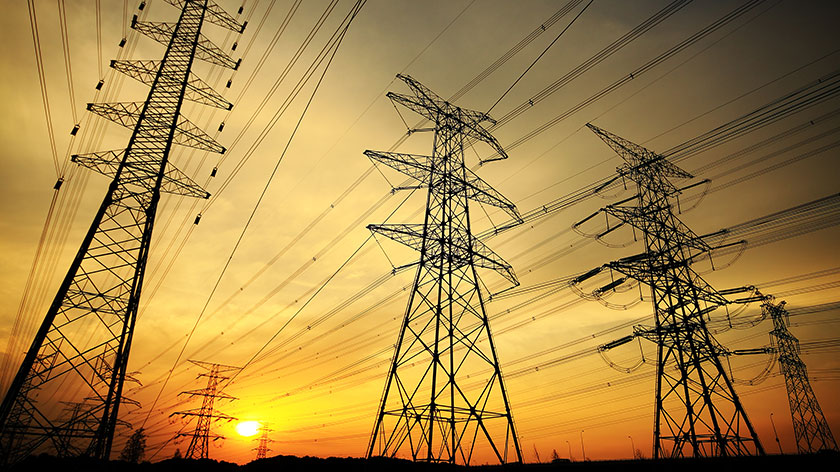
\includegraphics[width=0.65\linewidth]{Figuras/Ch01/fig1}

\end{frame}


\begin{frame}{Introdução}
	\begin{block}{Tensão}
		No dia a dia, não costumamos prestar muita atenção no conceito do \textbf{potencial}, mas pense sobre o seguinte fato:
		\begin{itemize}
			\item Tudo que \textbf{não} está no chão \textbf{pode} cair.
		\end{itemize}
		Pode soar óbvio e redundante falar isso, porém o \textbf{conceito físico} por trás do fenômeno é de \textbf{extrema importância}.

		\medskip

		O fato de que algo \textbf{pode} cair quer dizer que tem \textbf{potencial} para isso.
	\end{block}

	\centering
	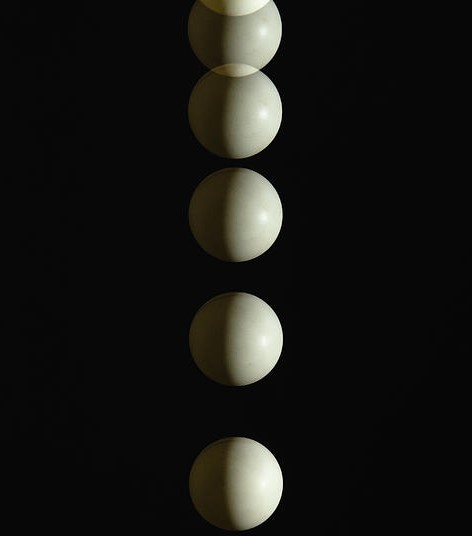
\includegraphics[height=0.4\textheight]{Figuras/Ch01/fig2}
\end{frame}


\begin{frame}{Tensão}
	\begin{block}{Potencial}
		\begin{itemize}
			\item O potencial pode soar um tanto abstrato, mas é, efetivamente, \textbf{energia acumulada}, que, por princípios naturais, quer ser dissipada, isso é, \textbf{liberada}.
			\item Mas repare que o objeto \textbf{não} deixa de ter energia quando chega ao chão, só vai ter menos... Portanto \textbf{ainda tem energia potencial} no chão.
			\item Para nós, que vivemos sobre o chão, não importa a energia total do objeto, só a energia relativa ao chão, portanto analisamos sua \textbf{diferença de potencial} (ddp).
		\end{itemize}
	\end{block}
\end{frame}


\begin{frame}{Tensão}
	\begin{block}{Diferença de potencial}
		\begin{itemize}
			\item O potencial relacionado a altura de um objeto que sofre efeitos gravitacionais é chamado \textbf{potencial gravitacional}.
			\item Dizemos, portanto, que uma bola com diferença de potencial gravitacional \textbf{maior do que zero} (em relação ao chão) \textbf{tende a cair}.
			\item Da mesma forma, aquilo que acende a lâmpada na sala é uma \textbf{diferença de potencial elétrico}, quantificada em \textbf{volt} ($ \si{\volt}=\si{\joule\per\coulomb} $).
			\item Trata-se da \textit{voltagem} ou \textit{tensão} a qual a lâmpada está sujeita.
		\end{itemize}
	\end{block}
\end{frame}


\begin{frame}{Tensão}
	\begin{block}{Nos fios}
		O preto representa o potencial \textit{negativo}, e o vermelho, o \textit{positivo}.
	\end{block}

	\centering
	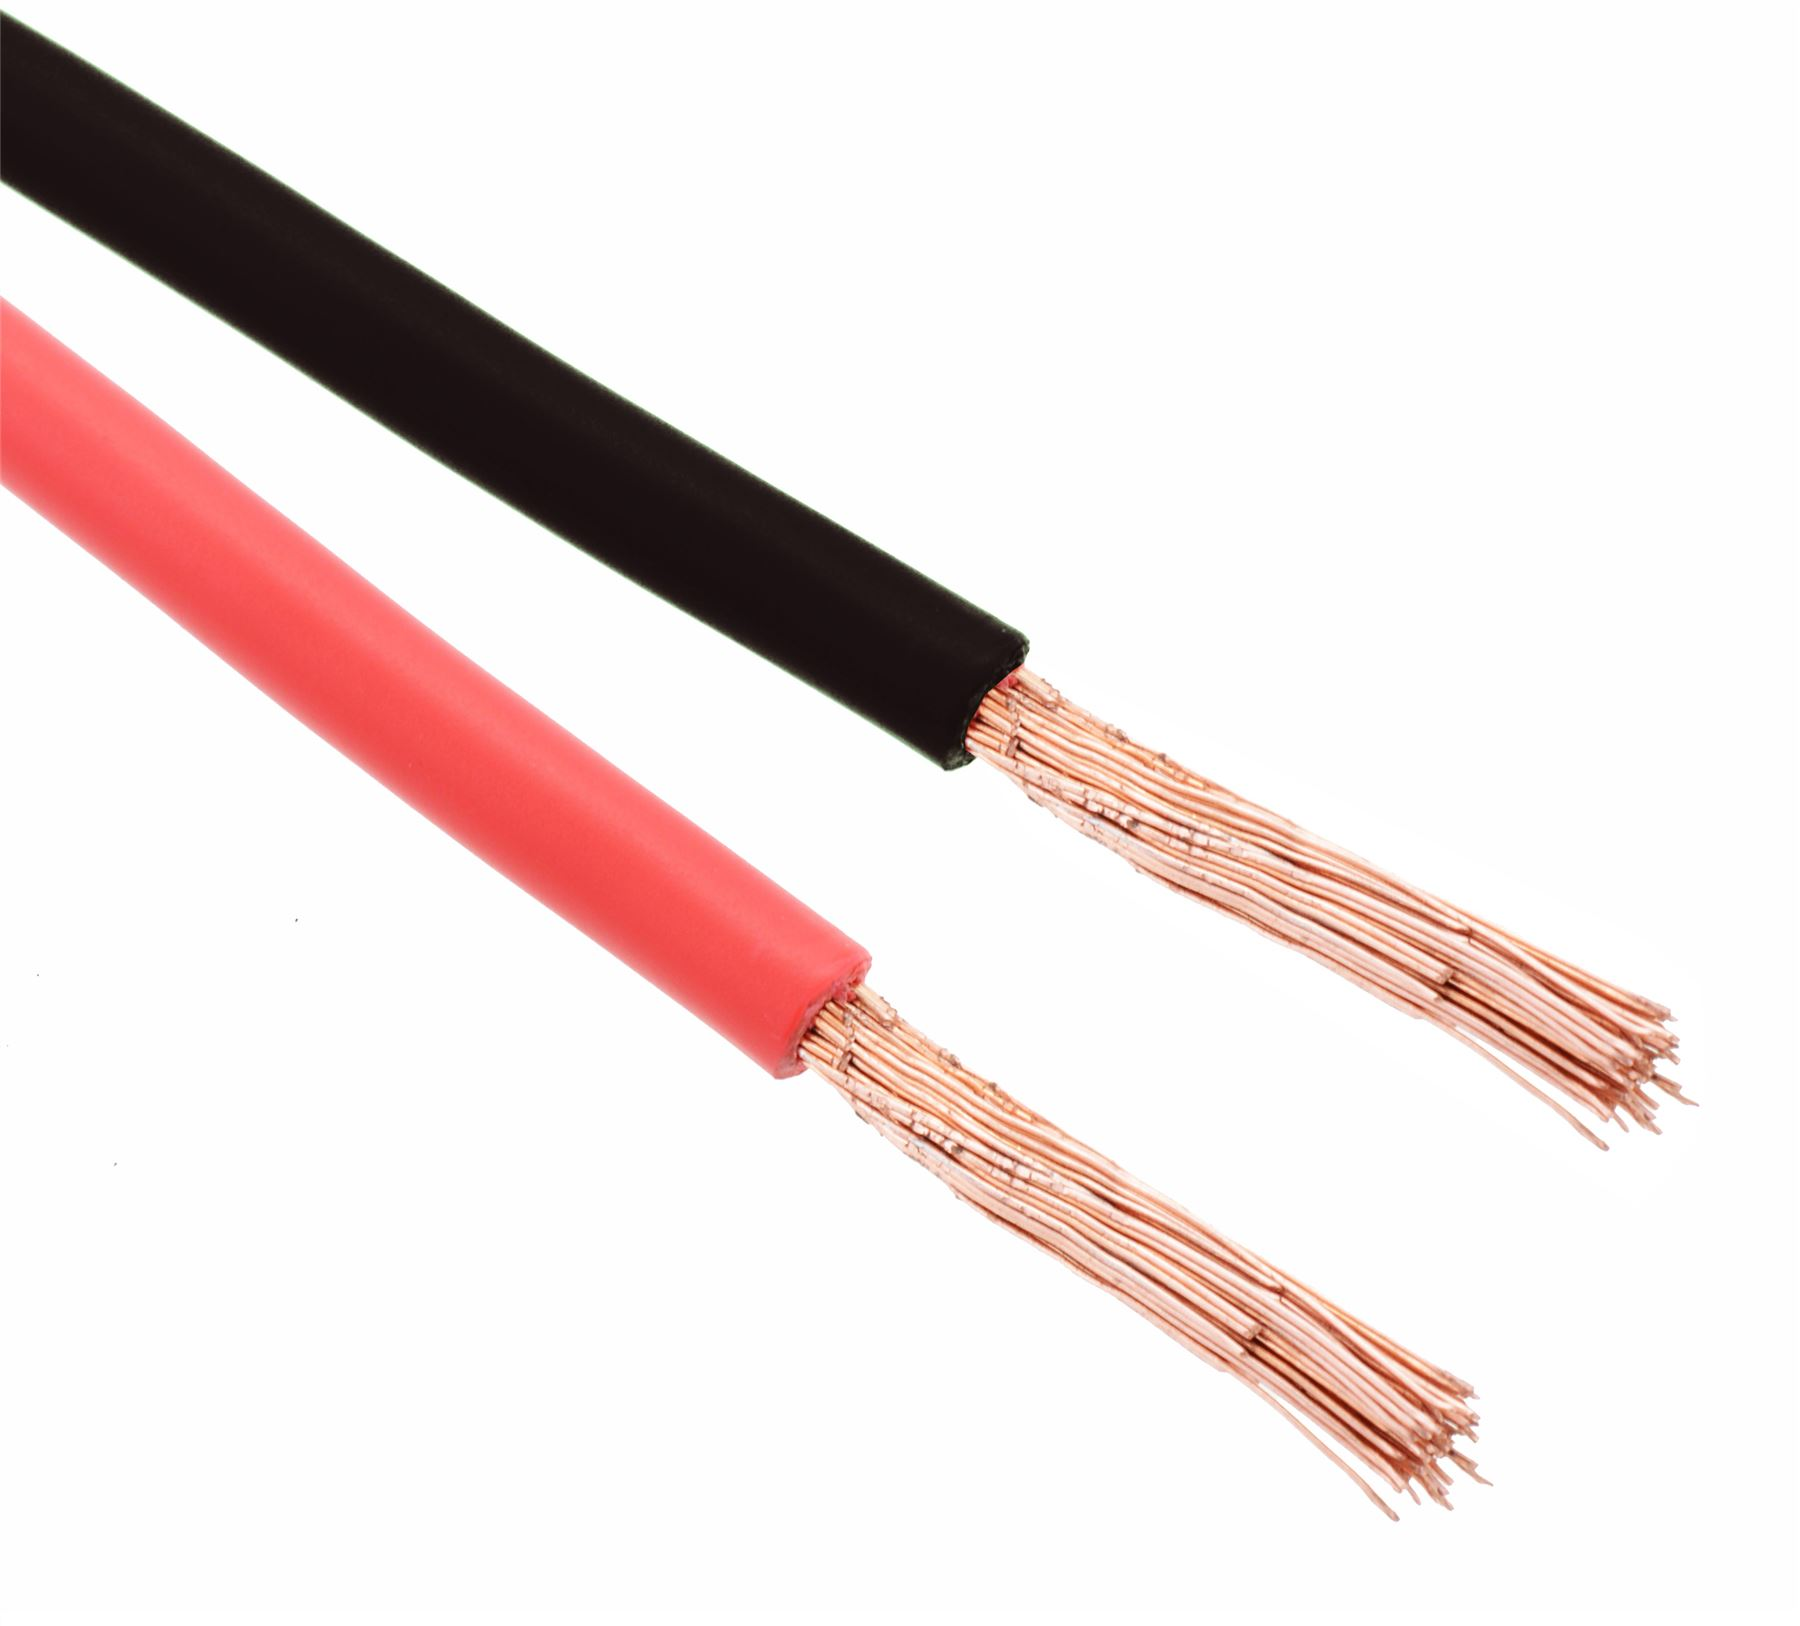
\includegraphics[width=0.6\linewidth]{Figuras/Ch01/fig6}

\end{frame}


\begin{frame}{Corrente}
	\begin{block}{Noção inicial}
		\begin{itemize}
			\item Esse ddp é produzido pelo \textbf{gerador} que, através de processos indutivos (relacionados aos ímãs), vai fornecer uma \textbf{diferença de potencial} entre pares de fios.
			\item Cada fio tem um \textbf{potencial associado} e, quando os juntamos, temos o \textbf{fluxo de energia} que acende uma lâmpada, ou carrega um celular.
			\item O fluxo de partículas que transportam a energia dentro dos fios chama-se \textit{corrente}.
			\item A corrente é medida em \textbf{ampère} ($ \si{\ampere}=\si{\coulomb\per\second} $).
		\end{itemize}
	\end{block}
\end{frame}


\begin{frame}{Corrente}
	\begin{block}{Realidade do fenômeno}
		\begin{itemize}
			\item Os átomos que compõem os objetos do dia a dia têm \textbf{elétrons}, que são partículas \textbf{móveis} e \textbf{carregadas}.
			\item Quando \textbf{não} há \textbf{ddp} no fio, os elétrons encontram-se em movimento \textbf{desordenado}, sem fluxo em uma direção definida.
		\end{itemize}
	\end{block}

	\bigskip

	\centering
	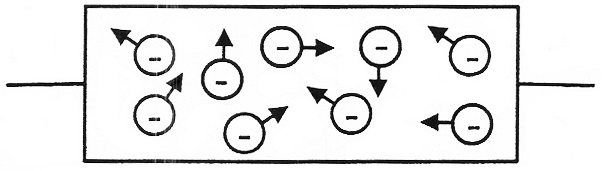
\includegraphics[width=0.65\linewidth]{Figuras/Ch01/fig8.1}

\end{frame}


\begin{frame}{Corrente}
	\begin{block}{Realidade do fenômeno}
		\begin{itemize}
			\item Quando aplicamos uma \textbf{ddp}, os elétrons tendem a fluir na direção da carga \textbf{oposta} a sua (do negativo para o positivo, portanto).
		\end{itemize}
	\end{block}

	\bigskip

	\centering
	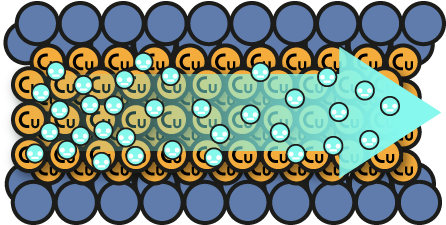
\includegraphics[width=0.65\linewidth]{Figuras/Ch01/fig8.2}

\end{frame}


\begin{frame}{Corrente}
	\begin{block}{Sentido}
		\begin{itemize}
			\item Por conta de fatores históricos, consideramos que a corrente flui do \textbf{positivo para o negativo}, isso é a \textbf{corrente convencional}.
			\item Na verdade, por terem carga negativa, os elétrons saem do \textbf{negativo para o positivo}, isso é a \textbf{corrente real}.
		\end{itemize}
	\end{block}

	\centering
	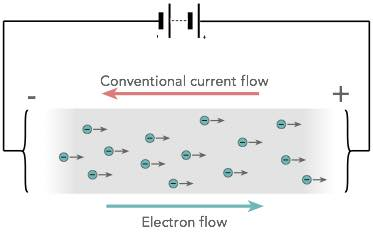
\includegraphics[width=0.65\linewidth]{Figuras/Ch01/fig8}

\end{frame}


\begin{frame}{Resistência}
	\begin{block}{Noção inicial}
		\begin{itemize}
			\item Lembre-se que qualquer material possui \textbf{limitações físicas}: quando um objeto cai, por exemplo, tem que atravessar o ar que está na atmosfera, e isso gera diversas \textbf{dificuldades} em sua movimentação.
			\item Num fio, devido às particularidades do condutor, os elétrons também lidam com obstáculos, e a dificuldade em sua movimentação é chamada \textit{resistência}.
			\item A resistência é medida em \textbf{ohm} (\si{\ohm}).
		\end{itemize}
	\end{block}
\end{frame}


\begin{frame}{Analogia - Fluidos}
	\begin{block}{}
		Podemos analisar a eletricidade como análoga aos fluidos:
		\begin{itemize}
			\item Imagine uma \textbf{caixa d'água} bem alta, cheia de água, isso é sua \textbf{bateria}, ou seu \textbf{gerador}, que fornece uma ddp.
			\item A água da caixa tem que passar pelas \textbf{tubulações} dela e, com isso, sofre as forças de \textbf{atrito}.
			\item A \textbf{altura da caixa} em relação ao chão é equivalente à \textbf{tensão aplicada} em fios.
			\item O \textbf{fluxo de água} (vazão) provocado pela altura é equivalente à \textbf{corrente}.
			\item A \textbf{dificuldade de passar pelos canos} é equivalente à \textbf{resistência}.
		\end{itemize}
	\end{block}
\end{frame}


\begin{frame}{Analogia - Fluidos}
	\centering
	%	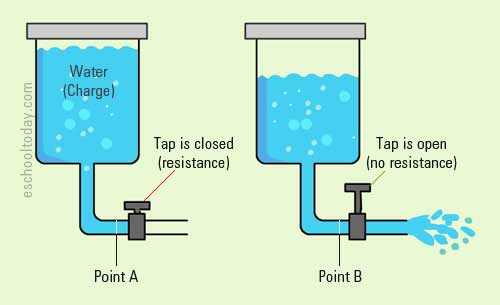
\includegraphics[width=0.9\linewidth]{Figuras/Ch01/fig3}
	\setmyunit{1.8cm}
	\begin{tikzpicture}
		\fill[blue] (0,0) -- ++(0,-3) -- ++(4,0) -- ++(0,0.5) -- ++(-1,0) -- ++(0,2.5) -- cycle;

		\draw (0,0) -- ++(0,-3) -- ++(4,0) ++(0,0.5) -- ++(-1,0) -- ++(0,2.5);

		\draw (0,0) -- +(0,0.5) (3,0) -- +(0,0.5);

		\draw[-Latex] (3,-2.75) ++(0,0.15) -- node[below=0pt] {Vazão} +(0.75,0);

		\draw[thick] (3.5,-2.5) -- ++(0,0.5) ++(0,0.4) circle (0.4);

		\foreach \x in {0,30,...,330}
		\draw (3.5,-1.6) ++(\x:0.35) -- +(\x:0.05);

		\draw (3.5,-1.6) -- +(25:0.4);

		\draw[decorate,decoration={brace,amplitude=10pt,mirror,raise=4pt}] (0,0) -- (0,-2.5) node[midway,left=15pt] {Altura};
	\end{tikzpicture}
\end{frame}


\begin{frame}{Relação entre conceitos}
	\begin{block}{Lei de Ohm}
		\begin{itemize}
			\item Podemos definir a resistência pela \textbf{lei de Ohm}, que relaciona a tensão aplicada com a corrente resultante e a resistência do meio.
			\item Sendo $ R $ a \textbf{R}esistência, $ I $ a \textbf{I}ntensidade da corrente e $ V $ a tensão aplicada (\textbf{V}oltagem), temos:\[ R=\dfrac{V}{I} \]
		\end{itemize}
	\end{block}

	\bigskip

	\centering
	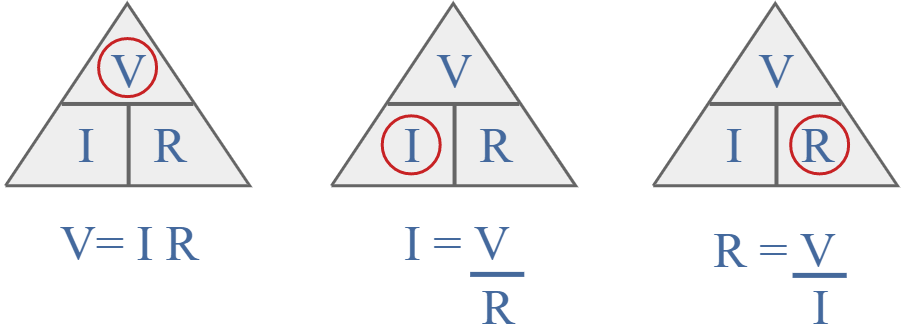
\includegraphics[width=0.7\linewidth]{Figuras/Ch01/fig9}
\end{frame}


\begin{frame}{Potência}
	\begin{block}{Noção inicial}
		\begin{itemize}
			\item Outro conceito importante é o da \textbf{potência}.
			\item Quando falamos de sistemas onde a energia é transferida, é interessante considerar a \textbf{capacidade de transferência} dessa energia.
			\item Além disso, sendo o \textit{tempo} \textbf{fator essencial} dos sistemas físicos, é útil incorporá-lo à nossa análise.
			\item Dessa forma, a \textit{potência} é a \textbf{energia fornecida pela corrente pelo tempo}, dada em \textbf{watt} ($ \si{\watt}=\si{\joule\per\second} $).
			\item A potência $ P $ relaciona-se à tensão, à corrente e à resistência pelas seguintes fórmulas:
			      \[ P=VI=\dfrac{V^{2}}{R}=RI^{2} \]
			\item Repare que as duas últimas fórmulas podem ser deduzidas a partir da lei de Ohm e da primeira fórmula.
		\end{itemize}

	\end{block}
\end{frame}


\begin{frame}{A eletricidade no dia a dia}
	\begin{block}{Tensão alternada}
		\begin{itemize}
			\item Infelizmente, as coisas no dia a dia não são tão simples quanto as ideias apresentadas.
			\item A eletricidade no Brasil, por exemplo, não tem uma ddp constante... É o que chamamos de \textbf{tensão variável}, ou \textbf{alternada}.
			\item Isso é consequência do \textbf{sistema de geração de energia}, e é algo que ocorre em \textbf{todo o mundo}, na verdade.
		\end{itemize}
	\end{block}
\end{frame}


\begin{frame}{A eletricidade no dia a dia}
	\begin{block}{Tensão alternada}
		Quando dizemos que a tensão é \textbf{alternada}, isso quer dizer que ela varia entre \textbf{positiva} e \textbf{negativa}. A tensão da tomada tem formato \textbf{senoidal}, como uma \textbf{onda}.
	\end{block}

	\centering
	\includegraphics[width=0.64\linewidth,page=2]{Figuras/Ch01/sinefunc}

\end{frame}


\begin{frame}{A eletricidade no dia a dia}
	\begin{block}{Tensão alternada}
		\begin{itemize}
			\item A tensão alternada é um pouco difícil de compreender, porém ela é muito útil, já que facilita muito a \textbf{transmissão} da energia, pois é somente assim que podemos usar \textbf{transformadores}.
			\item Também é interessante notar que \textbf{ainda há corrente} e \textbf{potência}.
		\end{itemize}
	\end{block}

\end{frame}


\begin{frame}{A eletricidade no dia a dia}
	\begin{block}{}
		Mas você já reparou que nos postes geralmente há mais de dois fios?
	\end{block}

	\centering
	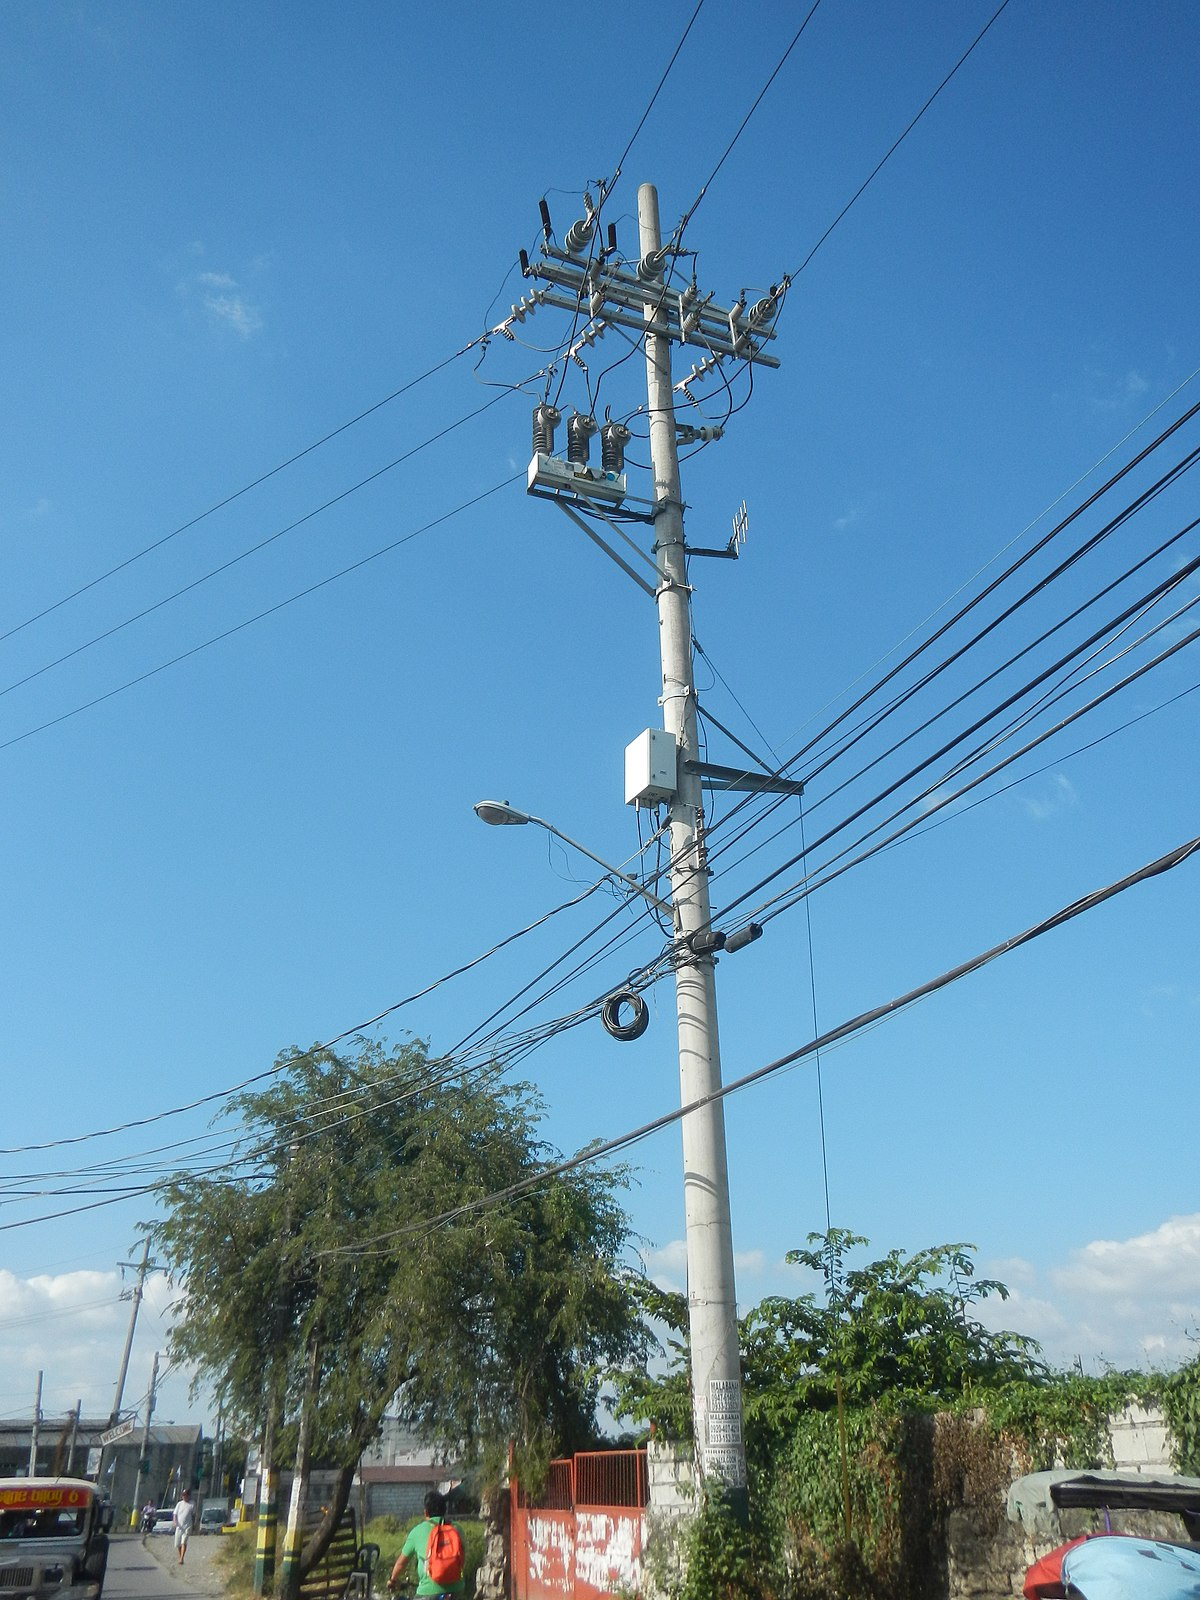
\includegraphics[height=0.7\textheight]{Figuras/Ch01/fig5}

\end{frame}


\begin{frame}{A eletricidade no dia a dia}
	\begin{block}{Potência}
		Acontece que transmitimos eletricidade em múltiplas \textit{fases}.

		\begin{itemize}
			\item Mas o que são estas?
		\end{itemize}

		Trata-se de uma forma \textbf{mais fácil} de \textbf{dividir} a \textbf{potência} necessária pra atender a uma região: quanto \textbf{mais potência} sua rede precisa, \textbf{mais fases} serão necessárias pra atender à demanda.
	\end{block}

\end{frame}



\begin{frame}{A eletricidade no dia a dia}
	\begin{block}{Potência}
		Cada um dos fios em cima do poste representa uma dessas fases, e todas tem um potencial relativo ao fio \textit{neutro}, que é um fio aterrado, e também tem potenciais relativos uma a outra.
	\end{block}

	\centering
	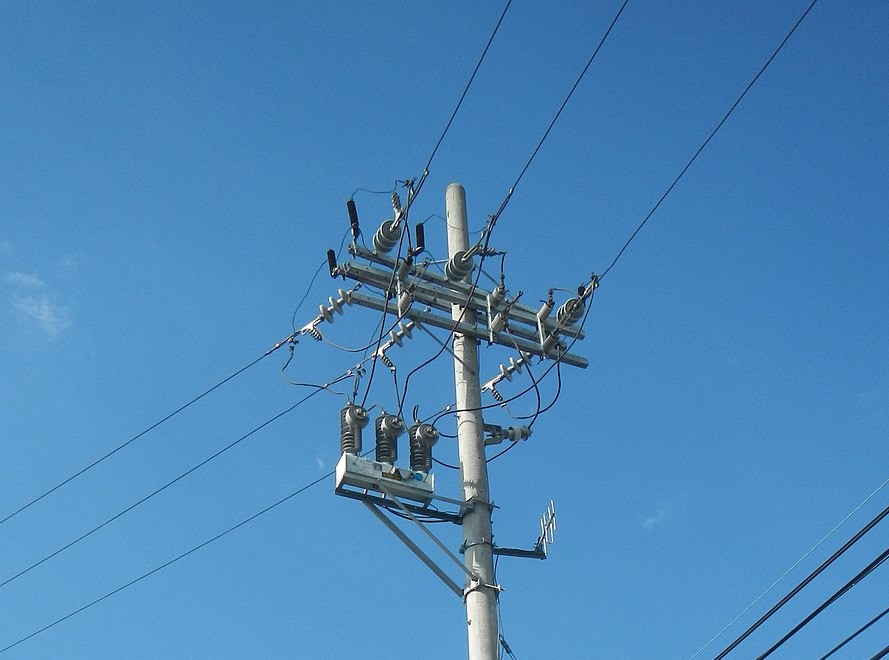
\includegraphics[height=0.6\textheight]{Figuras/Ch01/fig7}

\end{frame}


\begin{frame}{A eletricidade no dia a dia}
	\begin{block}{Potência}
		\begin{itemize}
			\item A potência em tensões alternadas é diferente da que vimos, por conta das particularidades do sistema.
			\item Toda potência calculada por $ P=VI $ em corrente alternada será dada em \textbf{volt-ampère} (\si{\va}), que é a unidade para \textbf{potência aparente}.
			\item Essa potência é a que um aparelho recebe, porém não necessariamente a que esse aparelho utiliza.
			\item Parte dessa potência é utilizada e descarregada em movimento, calor ou luz, e é chamada de \textbf{potência ativa}.
			\item O resto é a \textbf{potência reativa}, necessária para o funcionamento de motores, transformadores e reatores, por conta de suas propriedades indutivas.
		\end{itemize}
	\end{block}
\end{frame}


\begin{frame}{A eletricidade no dia a dia}
	\centering
	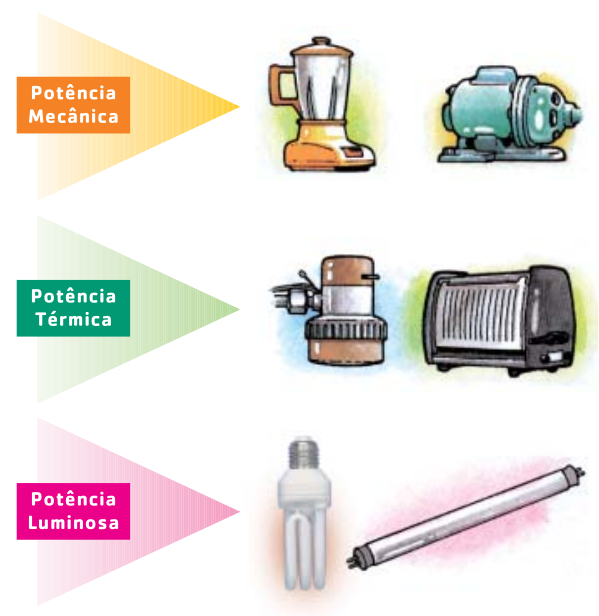
\includegraphics[width=0.65\linewidth]{Figuras/Ch01/fig11}

\end{frame}


\begin{frame}{A eletricidade no dia a dia}
	\centering
	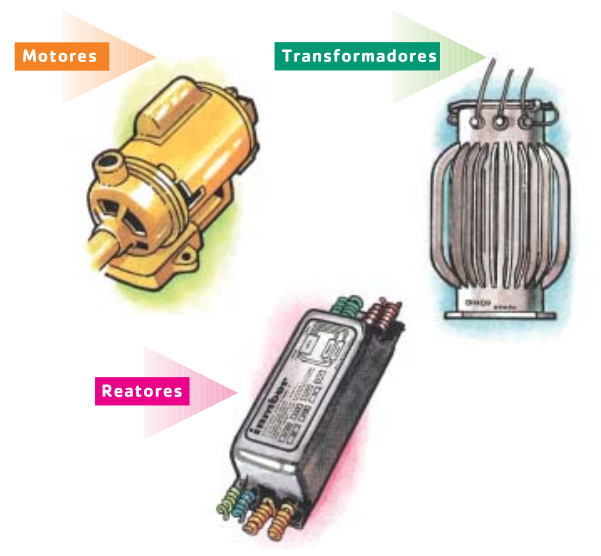
\includegraphics[width=0.7\linewidth]{Figuras/Ch01/fig12}

\end{frame}


\begin{frame}{A eletricidade no dia a dia}
	\begin{block}{Potência}
		\begin{itemize}
			\item A \textbf{potência ativa} é dada em \textbf{watt} (\si{\watt}), e é calculada multiplicando a potência aparente por um valor chamado \textit{fator de potência} ($ FP $):\[ PA=P\cdot FP \]
			\item O fator de potência é, simplesmente, a \textbf{porcentagem} da potência aparente que é potência ativa.
			\item Já a potência reativa é dada em \textbf{volt-ampère reativo} (\si{\var}), porém não é necessário utilizá-la nesse curso.
		\end{itemize}
	\end{block}
\end{frame}


\begin{frame}{A eletricidade no dia a dia}
	\begin{block}{Fator de potência}
		\begin{itemize}
			\item Se considerarmos os fatores matemáticos por trás das potências reativa e ativa, encontramos o fator de potência como o \textbf{cosseno do ângulo} formado no triângulo abaixo.
			\item Esse triângulo é conhecido como triângulo de potência, onde \[ FP=\cos{\varphi} = \cos{\left( \arctg{\dfrac{\text{Potência reativa}}{\text{Potência ativa}}}\right) } \]
		\end{itemize}
	\end{block}

	\centering
	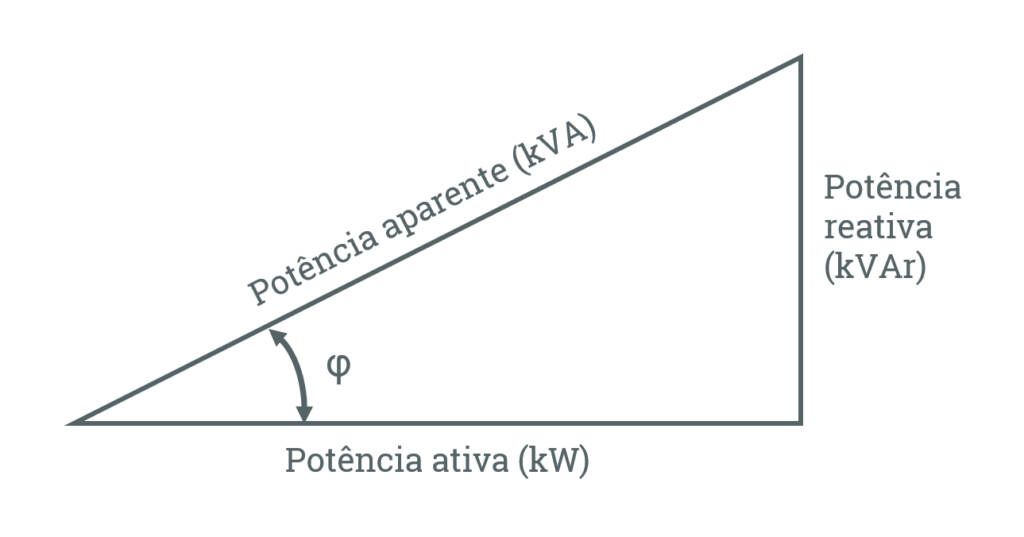
\includegraphics[width=0.7\linewidth]{Figuras/Ch01/fig13}
\end{frame}


\begin{frame}{A eletricidade no dia a dia}
	\begin{block}{Fator de potência}
		\begin{itemize}
			\item No Brasil, a Agência Nacional de Energia Elétrica - ANEEL - estabelece que o fator de potência deve ser maior do que \num{0,92}.
		\end{itemize}
	\end{block}

	\bigskip

	\centering
	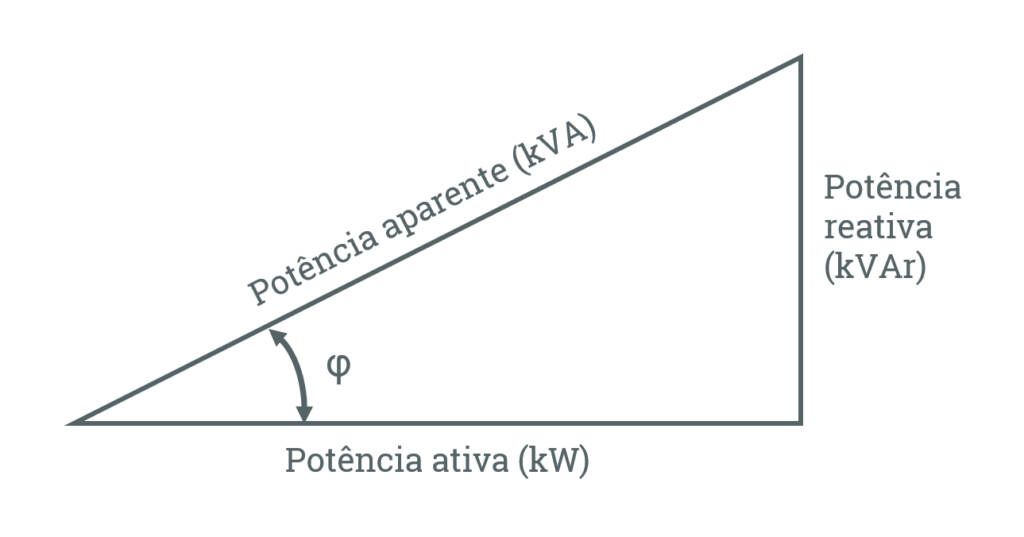
\includegraphics[width=0.7\linewidth]{Figuras/Ch01/fig13}
\end{frame}


\section*{Exercícios}
\frame{
	\frametitle{Exercícios}
	\begin{block}{}
		01. Imagine um circuito onde a corrente vale \SI{1}{\ampere} e a tensão vale \SI{50}{\volt}. Qual é a resistência a que o circuito está sujeito?

		\bigskip

		02. Considerando seus conhecimentos prévios e o que aprendeu nesse capítulo, deduza:

		\medskip

		(a) Para que servem os outros fios no poste?

		\medskip

		(b) Para que usamos transformadores?

		\medskip

		(c) Como a potência é afetada pelo número de fases? E a corrente?
	\end{block}
}

\section*{Referências}

\frame{
	\frametitle{Referências e Exercícios Complementares}
	\begin{itemize}
		\item CREDER, Hélio; Instalações Elétricas, 14ª edição, Editora LTC, Rio de Janeiro, 2004.
		\item Manual de Instalações Elétricas - Prysmian.
	\end{itemize}
	%\centering{\alert{Página 36 - \textbf{1.6.1 até 1.6.5, 1.6.17 até 1.6.19}}} \\
	%	\centering{\alert{Lista de exercícios 01}}
}